\documentclass[11pt,a4paper]{article}
%\usepackage{beamerarticle}

%\usefonttheme[onlymath]{serif}
\usepackage[ngerman]{babel}
\usepackage[utf8]{inputenc}
\usepackage[T1]{fontenc}
\usepackage{tikz}
\usetikzlibrary{positioning, arrows}
\usepackage{listings}
\usepackage{fancybox}
\usepackage{color}
\usepackage{hyperref}
\usepackage{fancyhdr}

\pagestyle{fancy}
\lhead{\today}
\author{Gruppe: SWT15-GKP}
\rhead{Author: KV}
\chead{Gruppe: SWT15-GKP}
%\cfoot{center of the footer!}
\renewcommand{\headrulewidth}{0.8pt}
%\renewcommand{\footrulewidth}{0.4pt}
\title{Universität Leipzig - Softwaretechnik Praktikum 2014/2015 \\  Entwurfsbeschreibung \\ zum Projekt: Ein kartenbasiertes “Multiplayer”-Spiel}

\begin{document}
\maketitle

\clearpage

\tableofcontents

\clearpage

\flushleft
\section{Allgemeines}
Im Rahmen des SWT-Praktikums wird ein kartenbasiertes Multiplayerspiel entwickelt, das es ermöglicht, ein an das alte Pacman angelehnte Computerspiel auf einem realen Kartenausschnitt zu spielen. Die entstehenden Highscores werden dann zu den jeweiligen Karten gespeichert um sich mit anderen Spielern messen zu können.


\section{Produktübersicht}
Der Nutzer kann online über die Spiele-Website auf das Programm zugreifen.
Dabei stehen dem Nutzer ein Suchfeld zum finden der gewünschten Spielumgebung zur Verfügung, wobei nur Städte ab einer bestimmten größe zugelassen sind, damit auf jedenfall eine spielbare Karte erstellt werden kann. Ebenfalls ist es möglich Spielorte über die Highscoreliste auswählen zu können. Desweiteren besteht die Möglichkeit die Spielfigur zu resetten und die Lautstärke über einen Regler anzupassen.
Hat man den Ort ausgewählt, wird das Spielfeld erzeugt und man kann ein neues Spiel beginnen. 

Man kann den Pucman nun mit Hilfe der Pfeiltasten steuern.
Es gibt unterschiedliche Geister, die durch ihr aussehen unterschieden werden können und sich anhand verschiedener Logiken bewegen. Fängt ein Geist den Spieler so wird dieser auf seinen Ausgangspunkt zurück gesetzt und die Anzahl seiner Leben wird um eins verringert. Falls keine Leben mehr übrig waren wird das Spiel beendet und der erreichte Highscore zusammen mit der Karten URI und dem Namen des Spielers abgespeichert

Während des Spielens werden die Möglichkeiten zur Veränderung der Kartenansicht  deaktiviert. Das Spielgeschehen ist durch einen Soundtrack unterlegt, der eine funktionale und inhaltliche Verbindung zwischen Bild und Musik generiert.
Desweiteren werden spielwichtige Informationen wie aktueller Highscore, die verbleibende Anzahl an Leben und die Möglichkeit direkt auf die Website des Spiels zugreifen zu können angezeigt.
\clearpage
\section{Grundsätzliche Struktur- und Entwurfsprinzipien}
Als grundsätzliche Programmiersprache haben wir uns für Java-Script entschieden. Wobei der Java-Scriptcode von einer HTML-Seite aufgerufen wird. Desweiteren benutzen wir Phaser als Gameframework.

Die von uns umgesetzte Web-Anwendung basiert auf einer Client-Server Architektur. Wir arbeiten also mit einem HTML-Server auf dem die Daten liegen, die vom Client abgefragt und an diesen übertragen werden. Diese Daten beinhalten auch den Gameblock, der dann vom Client ausgeführt wird. Darüber hinaus arbeiten wir mit der Googlemaps API, die alle wichtigen Funktionen zur Manipulation der Karte zur Verfügung stellt. Außerdem gibt es noch ein Map-Module, welches das Level aus den Geo-Daten erstellt, die mithilfe der Linked Geo Data API von OpenStreetMaps bezogen werden. Dazu kommt das Highscore-Module, welches für die Verwaltung der Highscores verantwortlich ist. Desweiteren kommt noch ein Datenserver hinzu, der die Highscores unter Verwendung eines Tripplestores speichert.\\
\begin{figure}[htb]
  \centering
  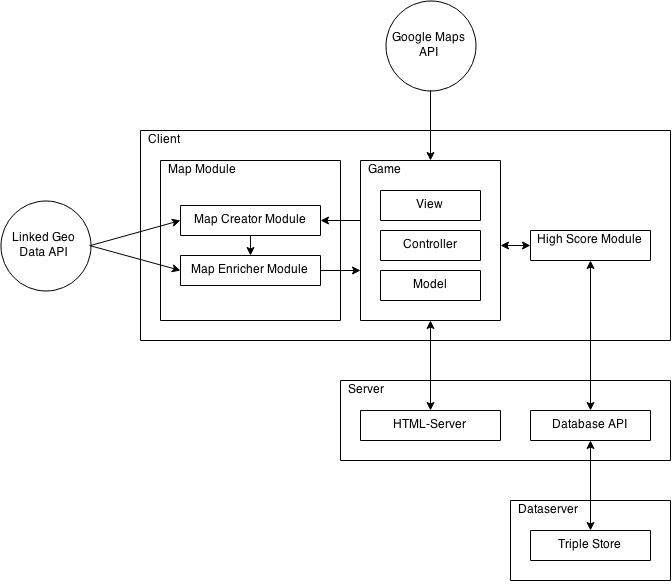
\includegraphics[scale=0.4]{arch.png}
%\caption{}
  \label{PNFs}
\end{figure} 



\section{Struktur- und Entwurfsprinzipien der einzelnen Pakete}
\subsection{Server} Vom Server werden die benötigten Spieldateien zur Verfügung gestellt und automatisch geladen. Desweiteren werden Highscoreanfragen und Manipulationen zwischen dem Dataserver und dem Client verarbeitet und anschließend weitergeleitet.

\subsection{Client}
Der Gameblock wird an das Model-View-Controller Prinzip angelehnt, welches durch die Nutzung von Phaser umgesetzt wird. \bigskip

Das Modell (model) enthält die darzustellenden Daten und ist von Präsentation und Steuerung unabhängig.\bigskip

Die Präsentationsschicht (view) ist für die Darstellung der benötigten Daten aus dem Modell und die Entgegennahme von Benutzerinteraktionen zuständig.\bigskip

Die Steuerung (controller) verwaltet die Präsentation, nimmt von ihr Benutzeraktionen entgegen, wertet diese aus und agiert entsprechend.\bigskip

Das Highscore Module verwaltet die Highscores der Spieler, d.h. es stellt Anfragen an den Server zum Triplestore und kann sie über den Server auch abfragen, falls sie im Spiel angezeigt werden sollen.\bigskip

Die Linked GeoData API extrahiert aus OpenStreetMap die Geo-Daten für das Erstellen des Spiel-Levels.\bigskip

Das Map Module besteht zum Einen aus dem Map Creator Module, welches lediglich den Graphen des Levels aus den Straßenzügen bildet, und zum Anderen aus dem Map Enricher Module, welches semantische Daten in die Kartenerstellung mit einbindet (z.B. Krankenhäuser, etc.). Das Map Module arbeitet mit den Geo-Daten die von der GeoData API geliefert werden.

\subsection{Google Maps API}

Das Herzstück der Anwendung ist die Googlemaps API, die das Anzeigen der Karte sowie das Suchen des eingegebenen Ortes übernimmt.
Die integrierten Steuerelemente sind bei der Suche nach einem  geeigneten Spielort verfügbar, danach werden die Elemente deaktiviert um  einen flüssigen Spielbetrieb zu gewährleisten.

\section{Datenmodell}

\begin{figure}[htb]
  \centering
  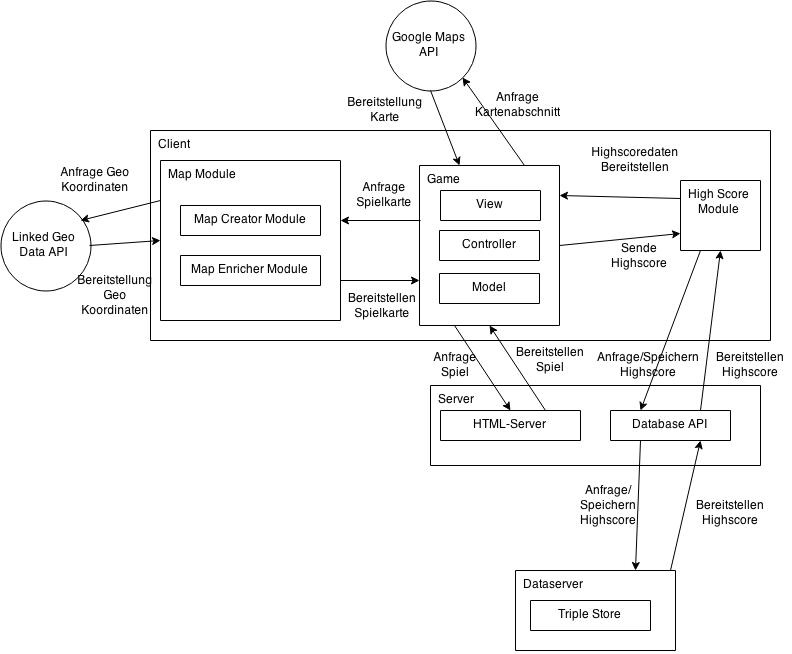
\includegraphics[scale=0.5]{Architecture.png}
  \label{PNFs}
\end{figure} 

\section{Testkonzept}
Jasmine ist eine freie Modultest-Bibliothek für JavaScript. Jasmine ist praktisch, da sie auf jeder JavaScript-fähigen Plattform ausführbar ist und keine Anpassung des Prüfsystems erfordert. Es ist eine sehr einfach gehaltene Testsprache und dadurch auch einfach lesbar
\section{Glossar}
Das Glossar wurde überarbeitet und als externes Dokument angefügt.
\end{document}